\documentclass[UTF8,aspectratio=169,11pt,fontset=fandol]{ctexbeamer}
\usepackage{amsmath,booktabs,graphicx,listings}
\definecolor{projectblue}{HTML}{1E4568}
\lstset{language=Python,basicstyle=\ttfamily\small,
  keywordstyle=\color{projectblue}\bfseries,commentstyle=\color{gray},
  backgroundcolor=\color{black!3},frame=single,rulecolor=\color{black!15},
  showstringspaces=false,columns=fullflexible,keepspaces=true,breaklines=true}
\setbeamercolor{structure}{fg=projectblue}
\setbeamercolor{frametitle}{fg=projectblue,bg=white}
\setbeamercolor{normal text}{fg=black,bg=white}
\setbeamertemplate{navigation symbols}{}
\setbeamertemplate{footline}{\hspace{1em}\scriptsize Micro-C 课程项目\hfill\insertframenumber\hspace{1em}\vspace{0.7em}}
\setbeamersize{text margin left=8mm,text margin right=8mm}
\setlength{\emergencystretch}{1em}
\title{基于深度学习的 Micro-C 接触矩阵处理}
\author{hycx233 \and onlysonder \and lanshuheng9-oss}
\date{2026 年 10 月}

\begin{document}
% A 开场约 70 秒；重点是学习任务与输入，不逐行讲代码。
\begin{frame}{把接触矩阵转化为两个深度学习任务}
\textbf{输入：}$128\times128$ 的单通道数值窗口，直接送入模型。
\vspace{0.7em}
\begin{columns}[T,onlytextwidth]
\begin{column}{0.47\textwidth}
\begin{block}{有标签：已知结构分类}
已知窗口 $\longrightarrow$ 小型 CNN\\[0.5em]
输出 OPCID / CHIN / CHID 三类分数。\\[0.6em]
\textbf{关心：}能否区分形态？\\
用测试指标、基线和解释图评价。
\end{block}
\end{column}
\begin{column}{0.47\textwidth}
\begin{block}{无标签训练：候选发现}
背景窗口 $\longrightarrow$ 自编码器\\[0.5em]
压缩到 32 维，再重建输入。\\[0.6em]
\textbf{关心：}哪些窗口难以重建？\\
高分窗口再用聚类与重复验证核查。
\end{block}
\end{column}
\end{columns}
\vspace{0.6em}
\small 数据规模：344 个已知结构，两个 WT 重复共 688 个分类窗口。\\[0.3em]
三条件轨道与条件比较用于展示和分析结果，复用同一套预处理。
\end{frame}

\begin{frame}[fragile]{从真实数据到模型输入：共用一个窗口接口}
\begin{block}{稀疏接触矩阵 $\longrightarrow$ 归一化与切窗 $\longrightarrow$ 模型张量}
10 bp 聚合到 100 bp，取 24 kb 上下文，统一为 $128\times128$。
\end{block}
\vspace{0.4em}
\begin{lstlisting}
state = load_sample(cache_dir, "WT_rep1")
window = extract_window(state, center)
x = torch.from_numpy(window["model"])
x = x[None, None]  # (1, 1, 128, 128)
\end{lstlisting}
\scriptsize 共享接口调用示意，省略导入；实现见 \texttt{src/preprocessing.py}。\par
\vspace{0.7em}
\normalsize
\textbf{两个关键选择：}
\begin{itemize}
\item 模型看 O/E 校正后的形态；强度比较使用另存的深度归一化数据。
\item 先按空间重叠分组，再划分训练/验证/测试（482/102/104 个窗口）。
\end{itemize}
\small 同一结构的重复和重叠窗口不跨集合，避免模型在测试时见过近似输入。
\end{frame}

% B / onlysonder：分类训练、评价边界与候选验证。
\begin{frame}{小型 CNN 输出三类分数}
\large 从共享窗口输入接触图，判断 OPCID、CHIN 或 CHID。

\vspace{0.7em}
\begin{center}
\small
$128\times128$ 窗口 $\;\longrightarrow\;$ 三个卷积模块（16/32/64 通道）\\[0.4em]
全局平均池化 $\;\longrightarrow\;$ OPCID / CHIN / CHID 三类分数
\end{center}

\vspace{0.7em}
\begin{itemize}
  \item 344 条已知结构使用 23,603 参数轻量 CNN；本项目未比较大型预训练编码器。
  \item 同一结构的两个重复以及共享划分标记为重叠的窗口不跨集合。
  \item 688 个窗口对应 344 条结构，不把重复窗口当成独立结构数。
\end{itemize}
\end{frame}

\begin{frame}[fragile]{训练只用训练集，轮次由验证集决定}
\large 加权交叉熵提高少数类在训练目标中的权重；Macro-F1 等权检查三类。

\vspace{0.45em}
\begin{lstlisting}
logits = model(features)
loss = criterion(logits, labels)
if training:
    optimizer.zero_grad(set_to_none=True)
    loss.backward()
    optimizer.step()
\end{lstlisting}

\small
Adam，学习率 $10^{-3}$，权重衰减 $10^{-4}$，dropout=0.3；seed=20260918。
按验证 Macro-F1 保存权重，patience=8。B 的独立 CPU 复跑在第 20 轮早停，最佳轮次为第 12 轮。
\end{frame}

\begin{frame}{固定测试集：CNN 尚未超过线性基线}
\large 多数类基线的 Accuracy 较高；展平矩阵的逻辑回归两项指标都高于 CNN。

\vspace{0.2em}
\begin{center}
\small
\begin{tabular}{lrrr}
\toprule
固定测试方法 & 样本数 & Accuracy & Macro-F1 \\
\midrule
小型 CNN & 104 & 0.5096 & 0.3454 \\
多数类（CHIN） & 104 & 0.7308 & 0.2815 \\
逻辑回归 & 104 & 0.8365 & 0.5644 \\
\bottomrule
\end{tabular}
\end{center}

\vspace{0.15em}
\begin{center}
\small
\begin{tabular}{lrrr}
\toprule
类别 & 测试样本数 & CNN F1 & 逻辑回归 F1 \\
\midrule
OPCID & 20 & 0.4062 & 0.8000 \\
CHIN & 76 & 0.6299 & 0.8931 \\
CHID & 8 & 0.0000 & 0.0000 \\
\bottomrule
\end{tabular}
\end{center}

\small
测试集为 52 个独立位置、每个两个 WT 重复。CNN 的 Macro-F1 高于多数类基线，
但两项指标均低于逻辑回归；三个方法都没有识别出 CHID。\\[0.3em]
每类另检查 3 个独立位置的 Grad-CAM；指标使用 B 本次复跑权重。
\end{frame}

\begin{frame}{47 个候选窗口合并后只有 10 个位置}
\large 邻近 1 kb 扫描窗口不能被当作独立复现。

\vspace{0.5em}
\begin{center}
\begin{tabular}{lrrr}
\toprule
类别 & 命中结构数（去重） & 已知结构数 & 去重召回 \\
\midrule
OPCID & 10 & 68 & 14.71\% \\
CHIN & 10 & 250 & 4.00\% \\
CHID & 1 & 26 & 3.85\% \\
\bottomrule
\end{tabular}
\end{center}

\vspace{0.4em}
\small
当前聚类没有满足既定疑似新簇规则：非噪声簇只有 4 个候选独立位置并含 297 个已知参考；
其余候选为 DBSCAN 噪声。WT rep2 的 O/E 相关和并排图待 \#9 运行后补入，不放宽规则。
\end{frame}

% C 部分约 3 分钟；按自编码器、有效像素损失、聚类判读和轨道实现展开。
\begin{frame}{自编码器候选发现}
\textbf{用背景窗口学习重建，再按误差筛选全基因组。}
\vspace{0.7em}

\centering
\large
$128\times128$ 接触图 $\longrightarrow$ 卷积编码器
$\longrightarrow$ 32 维表示 $\longrightarrow$ 解码器 $\longrightarrow$ 重建图
\normalsize
\vspace{0.9em}

\begin{columns}[T,onlytextwidth]
\begin{column}{0.46\textwidth}
\begin{block}{训练}
只使用 WT\_rep1 的背景窗口：17 个 train、4 个 val。\\[0.4em]
第 25 轮取得最低验证 masked MSE：\textbf{0.0223}。
\end{block}
\end{column}
\begin{column}{0.48\textwidth}
\begin{block}{筛选}
以 1 kb 步长扫描 4,642 个窗口，按重建误差前 1\% 保留
\textbf{47 个候选窗口}。
\end{block}
\end{column}
\end{columns}

\vspace{0.6em}
\small\raggedright 高重建误差只表示模型难以重建；候选仍需结合强度、已知结构、聚类和另一重复核查。
\end{frame}

\begin{frame}[fragile]{有效像素上的重建误差}
\textbf{缺失位置不作为零值目标，每个窗口按自己的有效像素数计算误差。}
\vspace{0.5em}

\begin{columns}[T,onlytextwidth]
\begin{column}{0.42\textwidth}
\centering
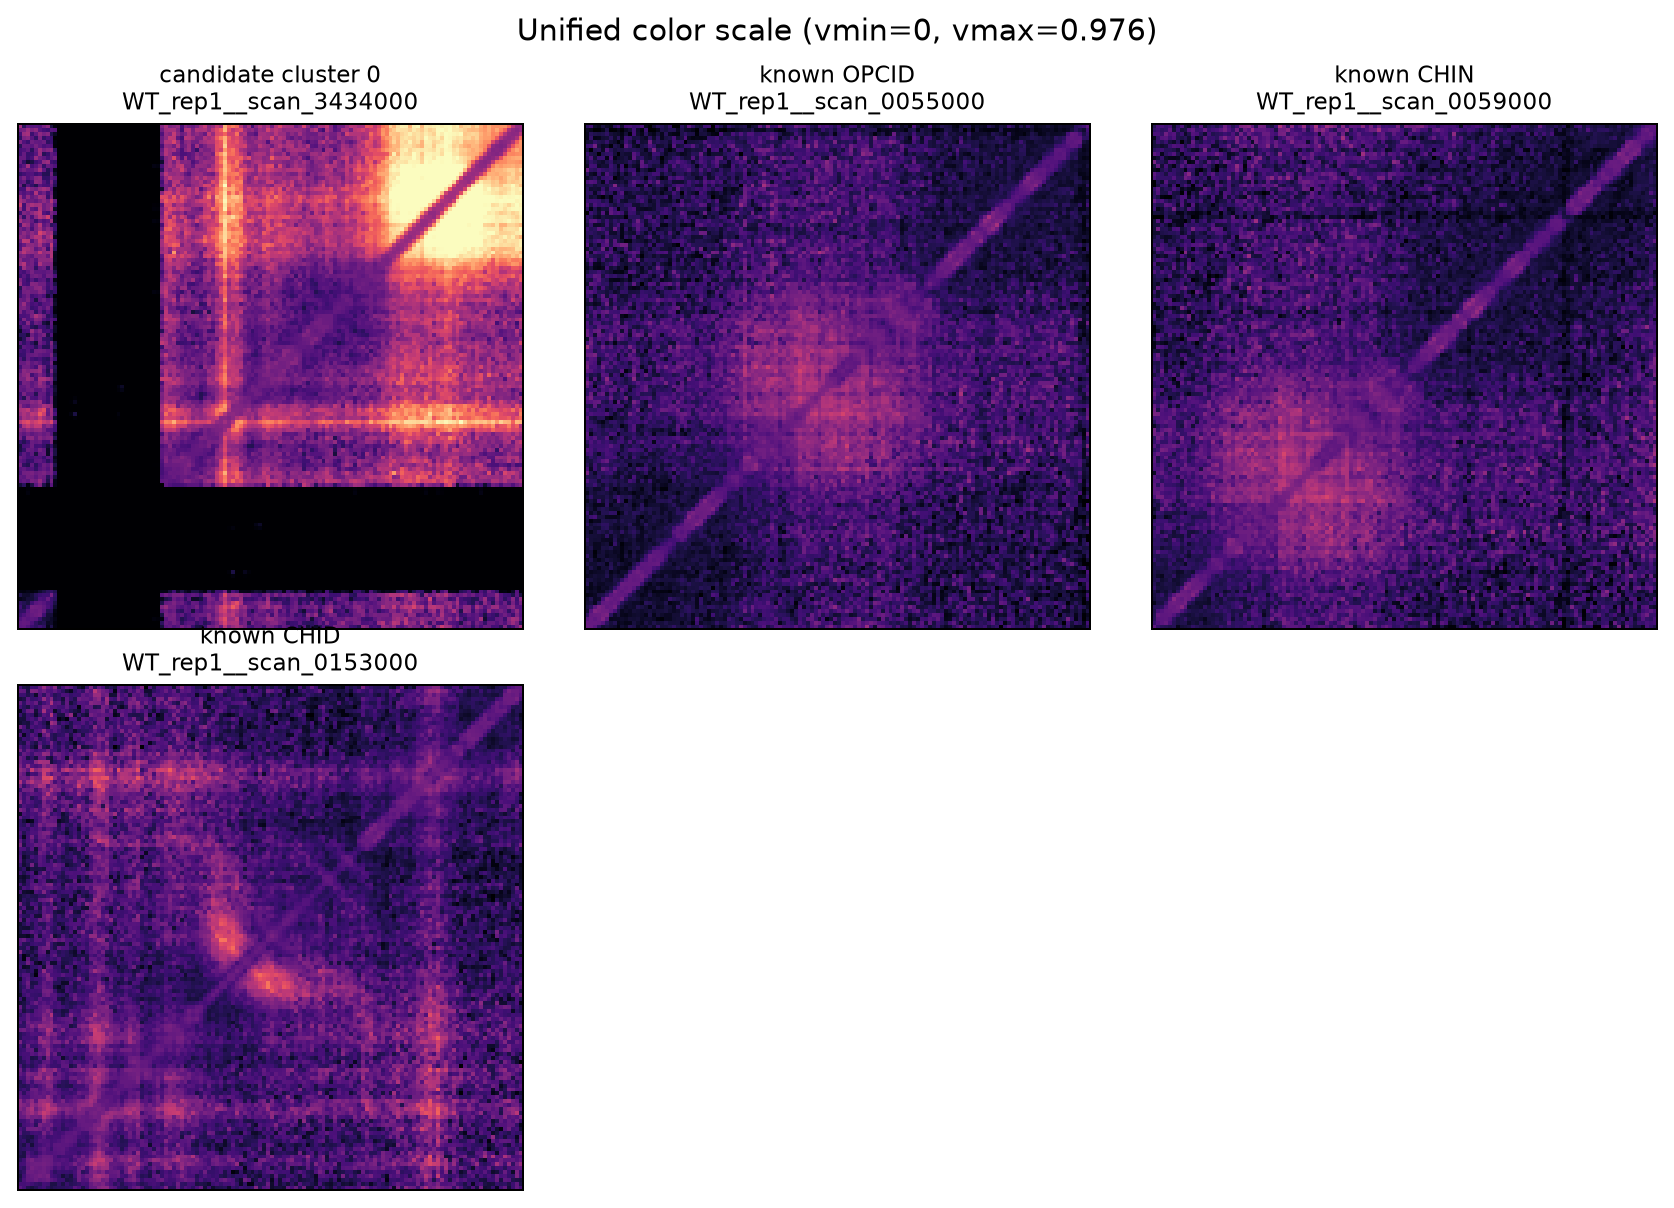
\includegraphics[width=\linewidth]{../results/clustering/cluster_representatives.png}\\[0.3em]
\scriptsize 灰色区域为数据缺口，不参与训练或打分。
\end{column}
\begin{column}{0.54\textwidth}
\begin{lstlisting}[basicstyle=\ttfamily\scriptsize]
valid_counts = window_mask.sum(dim=(1, 2))
squared_error = (prediction - target).square()[:, 0]
per_window = (squared_error * window_mask).sum(dim=(1, 2)) / valid_counts
\end{lstlisting}
\small
调用方先取逐窗口有效 mask 与上三角 mask 的交集，再传入
\texttt{masked\_mse}。每个窗口使用独立分母，避免缺口比例改变候选排序。
\end{column}
\end{columns}

\vspace{0.5em}
\small\textbf{结果检查：}误差与接触强度 Pearson 相关为 0.828；高分明显受强度影响，不能直接解释为新结构。
\end{frame}

\begin{frame}{候选聚类与独立位置}
\begin{columns}[T,onlytextwidth]
\begin{column}{0.64\textwidth}
\centering
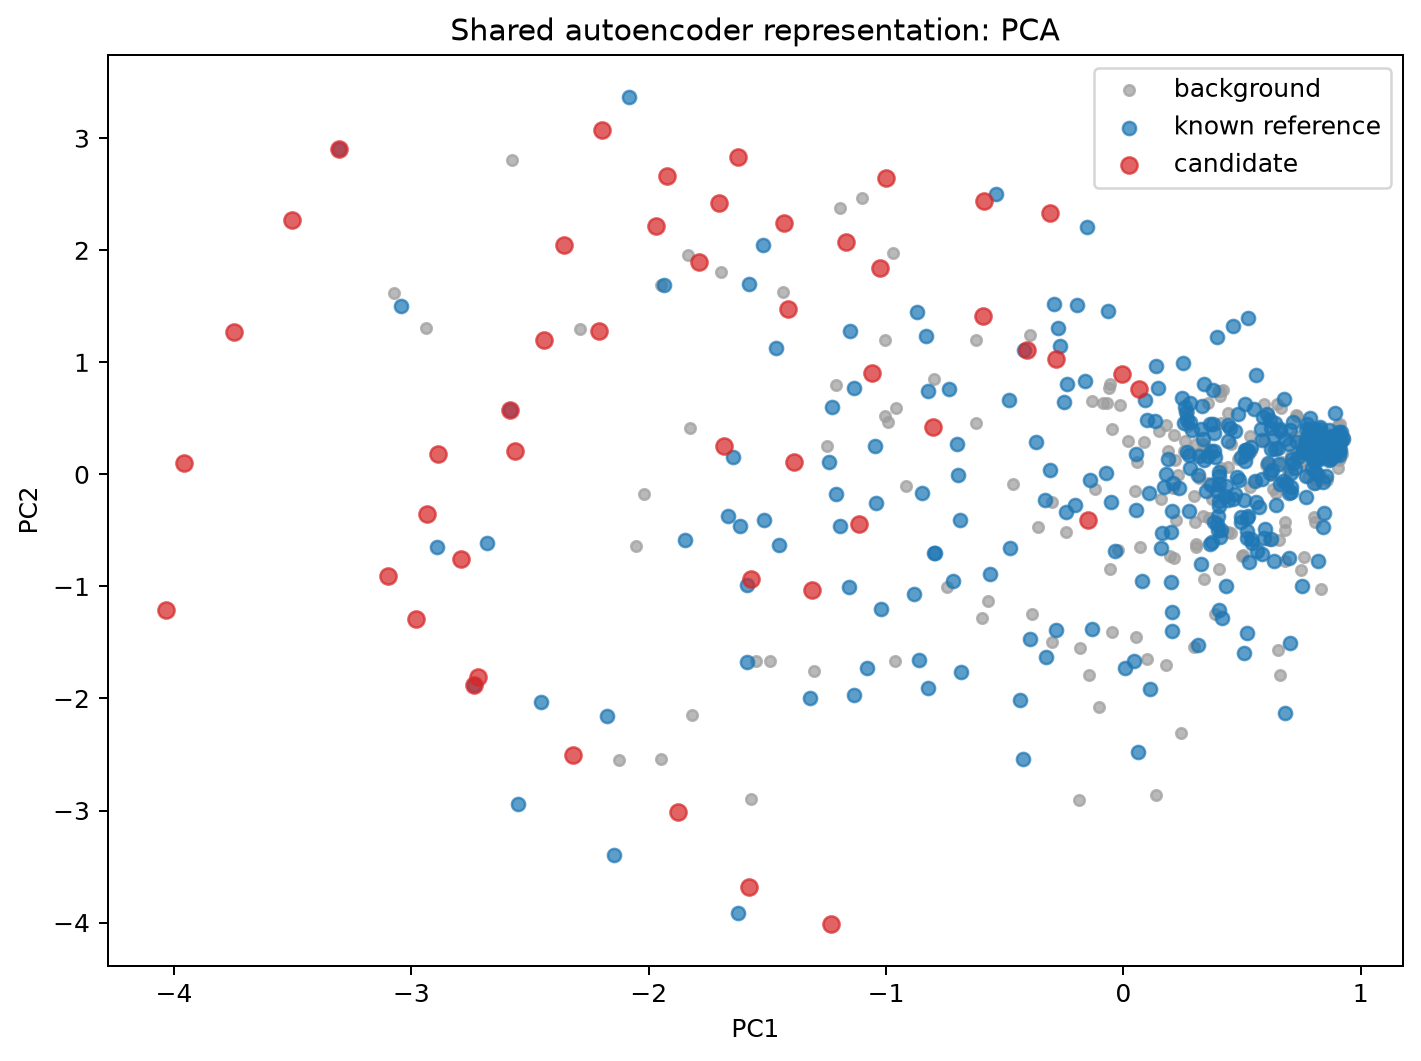
\includegraphics[height=0.60\textheight,keepaspectratio]{../results/clustering/pca_groups.png}\\[0.2em]
\scriptsize 图中显示前两个主成分；DBSCAN 实际使用 10 维白化 PCA 坐标。
\end{column}
\begin{column}{0.32\textwidth}
\small
\textbf{47 个候选窗口}\\[0.3em]
$\downarrow$ 合并重叠窗口\\[0.3em]
\textbf{10 个独立位置}

\vspace{0.8em}
唯一非噪声簇包含：
\begin{itemize}
\item 297 个已知参考
\item 9 个候选窗口
\item 4 个独立候选位置
\end{itemize}
\end{column}
\end{columns}

\vspace{0.4em}
\small\textbf{结论：}没有簇同时满足“至少 5 个独立位置、无已知参考、候选不与已知结构重叠”，本次不宣称发现新结构。
\end{frame}

\begin{frame}{三条件全基因组轨道}
\centering
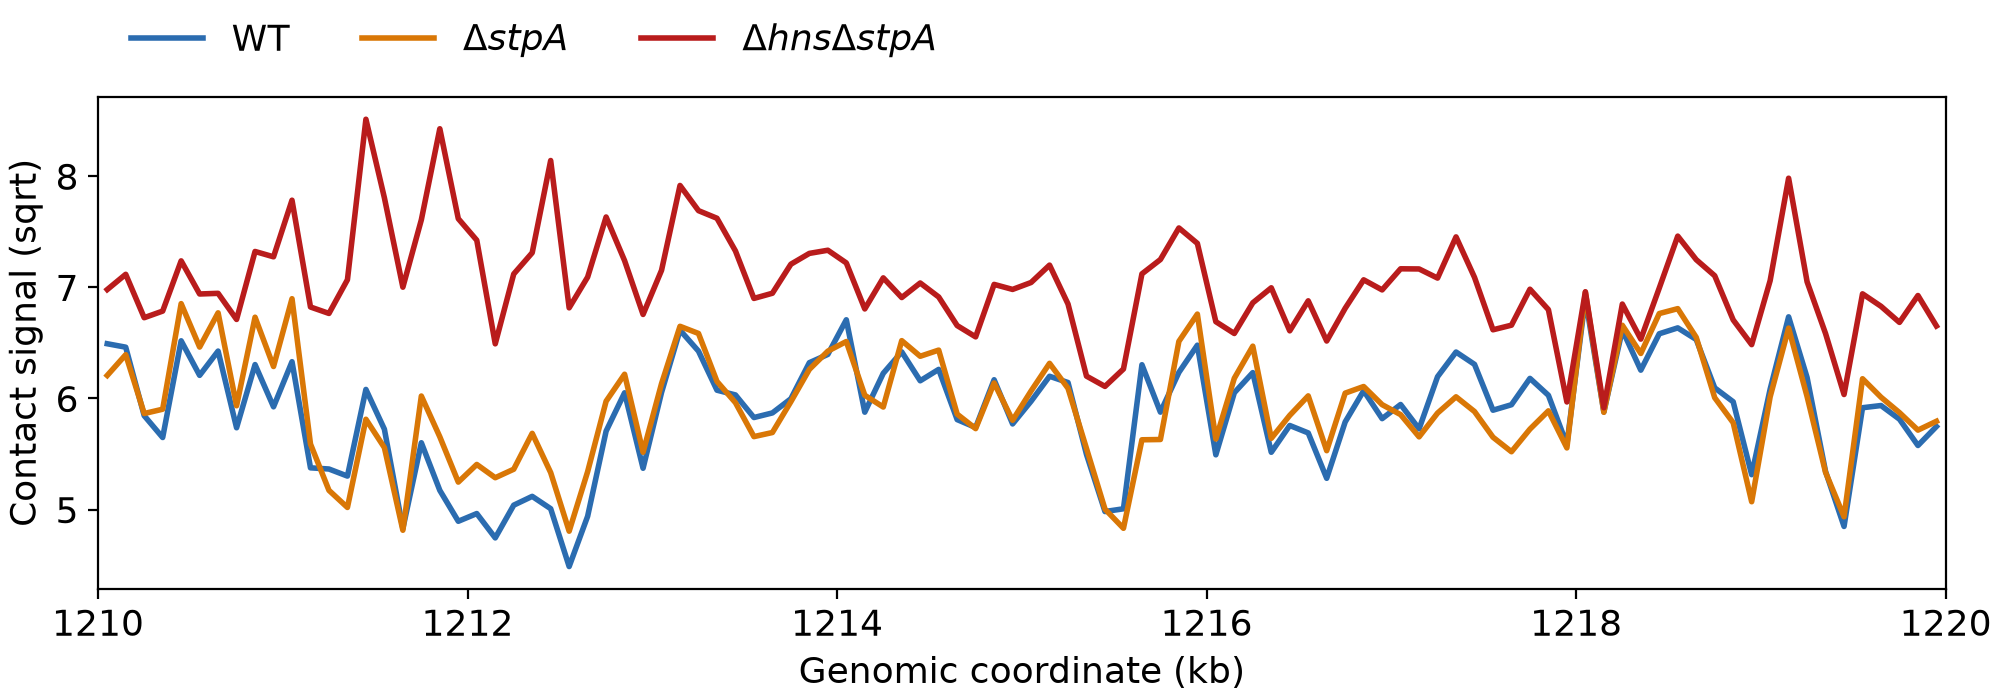
\includegraphics[width=0.98\textwidth]{../results/tracks/tracks_1210000_1220000_slide.png}\\[0.3em]

\raggedright\small
放大展示 1,210,000--1,220,000 bp 的条件均值；完整四面板见报告。\\[0.35em]
每个重复先按总接触量归一化；在线性尺度平均，再开平方显示。\\[0.35em]
全基因组连续输出 \textbf{465 张}四面板图，末图覆盖到 4,641,652 bp。\\[0.35em]
\textcolor{projectblue}{轨道用于定位和展示局部差异；曲线高低不等于统计显著性。}
\end{frame}

% A 差异与收束约 2 分钟；放在 B、C 讲解之后。
\begin{frame}{条件差异：比较结构内部的相对强度}
\textbf{344 个结构 $\times$ 2 个突变条件 = 688 行比较。}
\vspace{0.4em}

同一区间取六样本共同有效像素；条件内先平均两个重复，再与 WT 比较。
\[
F_c=\log_2\frac{\overline S_c}{\overline S_{\mathrm{WT}}},\qquad
b=\max\!\left(\log_2 1.25,\left|\log_2\frac{S_{\mathrm{WT},2}}{S_{\mathrm{WT},1}}\right|\right)
\]
\small 两个突变重复都越过同一侧参照带才标为一致增强或减弱。
\vspace{0.7em}

\centering
\begin{tabular}{lrrrr}
\toprule
条件 & 增强 & 减弱 & 带内 & 边界/不一致 \\
\midrule
$\Delta stpA$ & 217 & 6 & 94 & 27 \\
$\Delta hns\Delta stpA$ & 182 & 10 & 92 & 60 \\
\bottomrule
\end{tabular}
\vspace{0.6em}

\raggedright\small 描述性参照，不是显著性检验；12 个低覆盖结构留在全表，不用于代表案例。
\end{frame}

\begin{frame}{实例：CHIN\_126 在 $\Delta stpA$ 下重复一致增强}
\centering
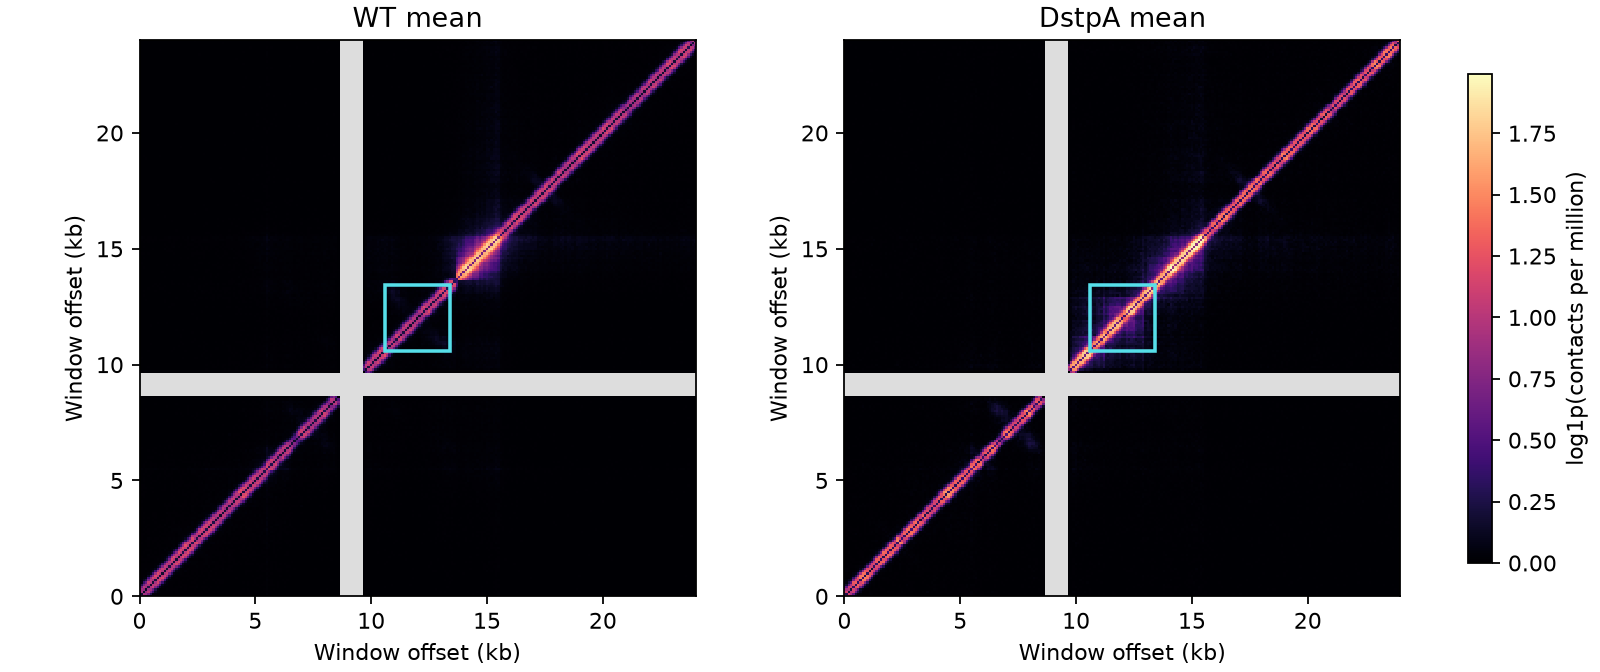
\includegraphics[width=0.94\textwidth]{../results/differences/figures/CHIN_126_DstpA_slide.png}\\[0.3em]
\small 青框为量化区间；灰色为共同无效区域。均值约为 WT 的 \textbf{2.504 倍}。\\[0.4em]
\small 两重复相对 WT 的 $\log_2$ 比为 1.306、1.342，均高于参照带上界 0.322。
\end{frame}

\begin{frame}{结论与解释范围}
\begin{block}{已完成的比较}
\normalsize 共享流程连接分类、候选发现、465 张轨道图及 688 行条件比较。\\
同一条件下既有增强也有减弱，代表案例同时保留稳定与边界结果。
\end{block}
\vspace{0.5em}
\begin{itemize}
\item 47 个高分候选仅对应 10 个独立位置；目前没有满足规则的疑似新簇。
\item 深度归一化后的相对增强，不等于细胞内绝对接触总量增加。
\item 两个重复用于描述性对照，双缺失结果不归因于单个因子。
\end{itemize}
\vspace{0.6em}
\small\textcolor{projectblue}{阶段稿：最终录制前，在 B 的章节补齐分类测试、基线/解释图与跨重复验证结论。}
\end{frame}

\end{document}
